% !TeX root = RJwrapper.tex
\title{Newsflow: An R package for analyzing content homogeneity and news
diffusion using computational text analysis}
\author{by Kasper Welbers, Wouter van Atteveldt}

\maketitle

\abstract{
Given the sheer amount of news sources in the digital age (e.g.,
newspapers, blogs, social media) it has become difficult to determine
where news is first introduced and how it diffuses across sources. We
introduce Newsflow: an R package for analyzing content homogeneity and
diffusion patterns using computational text analysis. The content of
news messages is compared using techniques from the field of information
retrieval, similar to plagiarism detection. By using a sliding window
approach to only compare messages within a given time distance, it is
made easy to compare many sources over long periods of time.
Furthermore, the package introduces an approach for analyzing the news
similarity data as a network, and includes various functions to analyze
and visualize this network.
}

\section{Introduction}

The news diffusion process in the digital age involves many
interdependent sources, ranging from news agencies and traditional
newspapers to blogs and people on social media
\citep{meraz11, paterson05, pew10}. We offer the \texttt{Newsflow} R
package\footnote{R is an open-source statistical software package
  (\url{https://www.r-project.org/}).} as a toolkit to analyze the
homogeneity and diffusion of news content using computational text
analysis. This analysis consists of two steps. First, techniques from
the field of information retrieval are used to measure the similarity of
news messages (e.g., addressing the same event, containing identical
phrases). Second, the temporal order in which messages are published is
used to analyze consistent patterns in who follows whom.

The main contribution of this package lies in the specialized
application of document similarity measures for the purpose of comparing
news messages. News is a special type of information in the sense that
it has a time dimension---it quickly loses its relevance. Therefore, we
are often only interested in the similarity of news documents that
occured within a short time distance. By restricting document
comparisons to a given time distance, it becomes possible to compare
many documents over a long period of time, but available document
comparison software generally does not have this feature. We therefore
offer the \texttt{documents.window.compare} function which compares
documents using a sliding window over time. In addition, this package
offers tools to aggregate, analyze and visualize the document similarity
data.

The primary intended audience of this package is scholars and
professionals in fields where the impact of news on society is a prime
factor, such as journalism, political communication and public relations
\citep{baum08, boczkowski07, ragas14}. To what extent the content of
certain sources is homogeneous or diverse has implications for central
theories of media effects, such as agenda-setting and the spiral of
silence \citep{bennett08, blumler99} Identifying patterns in how news
travels from the initial source to the eventual audience is important
for understanding who the most influential ``gatekeepers'' are
\citep{shoemaker09}. Furthermore, the document similarity data enables
one to study news values \citep{galtung65} by analyzing what elements of
news predict their diffusion rate and patterns.

The package is designed to appeal to scholars and professionals without
prior experience in computational text analysis. This vignette covers
the entire chain from processing raw data---written text with source and
date information---to analyzing and visualizing the output. It points to
relevant software within and outside of R for pre-processing written
texts, and demonstrates how to use the core functions of this package.
For more advanced users there are additional functions and parameters to
support versatility. \texttt{Newsflow} is completely open-source to
promote active involvement in developing and evaluating the methodology.
The source code is available on Github---\url{https://github.com/masked}
(repository hidden for review). All data used in this vignette is
included in the package for easy replication.

The structure of this vignette is as follows. The first part discusses
the data preparation. There are several choices to be made here that
determine on what grounds the content of documents is compared. The
second part shows how the core function of this packages,
\texttt{documents.window.compare}, is used to calculate document
similarities for many documents over time. The third part demonstrates
functions for exploring, aggregating and visualizing the document
similarity data. Finally, conclusions regarding the current version of
the package and future directions are discussed.

\section{Preparing the data}

To analyse content homogeneity and news diffusion using computational
text analysis, we need to know \emph{who} said \emph{what} at
\emph{what time}. Thus, our data consists of messages in text form,
including meta information for the source and publication date of each
message. The texts furthermore need to be pre-processed and represented
as a \emph{document-term matrix} (DTM). This section first discusses
techniques and refers to existing software to pre-process texts and
create the DTM, and reflects on how certain choices influence the
analysis. Second, it shows how the source and date information should be
organized. Third, it discusses several ways to filter and weight the DTM
based on word statistics.

\subsection{Pre-processing texts and creating the DTM}

A DTM is a matrix in which rows represent documents, columns represent
terms, and cells indicate how often each term occurred in each document.
This is referred to as a \emph{bag of words} respresentation of texts,
since we ignore the order of words. This simplified representation makes
analysis much easier and less computationally demanding, and as research
has shown: ``a simple list of words, which we call unigrams, is often
sufficient to convey the general meaning of a text''
\citep[6]{grimmer13}.

As input for this package, the DTM has to be in the
\texttt{DocumentTermMarix} class of the \texttt{tm} package. This is a
popular R package for text mining, or computational text analysis, which
also contains functions to create a DTM based on raw text in various
formats. We also recommend the \texttt{RTextTools} package, which has
the \texttt{create\_matrix} function that wraps various \texttt{tm}
functions for creating a DTM into a single convenient function. For
example, see the following DTM, created with the \texttt{create\_matrix}
function.

\begin{Schunk}
\begin{Sinput}
document1 = 'Socrates is human'
document2 = 'Humans are mortal'
document3 = 'Therefore, Socrates is mortal'
dtm = RTextTools::create_matrix(textColumns = c(document1,document2,document3), 
                                minWordLength = 1, removeStopwords = F)

as.matrix(dtm)
\end{Sinput}
\begin{Soutput}
#>     Terms
#> Docs are human humans is mortal socrates therefore
#>    1   0     1      0  1      0        1         0
#>    2   1     0      1  0      1        0         0
#>    3   0     0      0  1      1        1         1
\end{Soutput}
\end{Schunk}

Based on the representation of texts in the DTM, the similarity of
documents can be calculated as the similarity of row vectors. However,
as seen in the example, this approach has certain pitfalls if we simply
look at all words in their literal form. For instance, the words
``human'' and ``humans'' are given separate columns, despite having
largely the same meaning. As a result, this similarity of the first two
texts is not recognized. Also, the words ``are'', and ``is'' do not have
any substantial meaning, so they are not informative and can be
misleading for the calculation of document similarity. There are various
techniques to filter and transform words that can be used to mend these
issues. In addition, we can use these techniques to steer on what
grounds documents are compared.

\begin{itemize}
\item
  First of all, it is advisable to make all terms lowercase, and reduce
  terms to their root using stemming or lemmatizing\footnote{Stemming
    and lemmatization are both techniques for reducing words to their
    root, or more specifically their stem and lemma. This is used to
    group different forms of the same word together. Without going into
    specifics, lemmatization is a much more computationally demanding
    approach, but generally gives better results. Especially for richly
    inflicted languages such as German or Dutch it is highly recommended
    to use lemmatization instead of stemming.}. Thus, ``Hope'',
  ``hoped'', ``hoping'', etc. all become ``hope''. This is because we
  are interested in the meaning of these terms, and not the specific
  form in which they are used.
\item
  Second, one should filter out irrelevant words. Very common words,
  stopwords and boilerplate words contain little or no relevant
  information about news items. Very rare terms, while ignored in many
  computational text analysis approaches, are particularly informative
  for our current purpose, and should be kept.
\item
  Third, It is also possible to specifically select or filter out only
  certain types of words by using part-of-speech tagging\footnote{Part-of-speech
    tagging is a technique that identifies types of words, such as
    verbs, nouns and adjectives.}. For instance, to compare whether
  documents address the same event one can focus on nouns and proper
  names.
\item
  Finally, an alternative approach is to combine words into N-grams
  (i.e.~sets of N consecutive words). This way the comparison of
  documents focuses more on similarity in specific segments of text,
  which is useful if the goal is to trace whether sources literally copy
  each other (in which case most other pre-processing steps can be
  skipped).
\end{itemize}

All mentioned techniques except for lemmatization and part-of-speech
tagging are available in the \texttt{tm} package and in the
\texttt{create\_matrix} function of the \texttt{RTextTools} package. To
use lemmatization or part-of-speech tagging there are several free to
use grammar parsers, such as
\emph{CoreNLP* for English [@corenlp] and *Frog} for Dutch
\citep{bosch07}\footnote{To create a DTM based on externally
  pre-processed documents, one can use the base function \texttt{xtabs}
  to create a sparse matrix and the \texttt{as.DocumentTermMatrix}
  function from the \texttt{tm} package to transform this matrix to the
  \texttt{DocumentTermMatrix} class.}.

For this vignette, data is used that has been preprocessed with the
Dutch grammar parser Frog. The data is based on a recent study on the
influence of a Dutch news agency on the print and online editions of
Dutch newspapers in political news coverage (Author citation,
forthcoming). The terms have been lemmatized, and only the nouns and
proper names of the headline and first five sentences (that generally
contain the essential who, what and where of news) are used. By focusing
on these elements, the analysis in this study focused on whether
documents address the same events. This data is also made available in
the package as demo data, in which the actual nouns and proper names
have been substituded with indexed part-of-speech tags.

\begin{Schunk}
\begin{Sinput}
data(dtm)
as.matrix(dtm[1:3,1:5])
\end{Sinput}
\begin{Soutput}
#>           Terms
#> Docs       person.688 noun.1516 location.119 organization.323 person.493
#>   35573532          0         0            0                0          0
#>   35573536          0         0            0                0          0
#>   35573539          0         0            0                0          0
\end{Soutput}
\end{Schunk}

\subsection{Organizing document meta information}

In addition to the DTM, we need meta information for each document. This
should be structured as a data frame with at least two columns. The
first column contains the document names, and should match with the
rownames (i.e.~document names) of the DTM. The second column contains
the publication date of the document, which should be in the
\texttt{Date} or \texttt{POSIXct} class. For easy compatibility with the
functions offered in this package, it is recommended to label these
columns ``document\_id'' and ``date''. Any additional columns in the
meta data.frame can be used in the analysis to aggregate and visualize
results. Here it is recommended to have at least a column containing the
source of the document, labeled ``source''.\footnote{``document\_id'',
  ``date'' and ``source'' are the default labels used in several
  functions to interpret the meta information. Note that these defaults
  can always be changed using the function parameters. Using the default
  labels only serves as a convenience.}

\begin{Schunk}
\begin{Sinput}
data(meta)
head(meta,3)
\end{Sinput}
\begin{Soutput}
#>   document_id                date     source sourcetype
#> 1    35573532 2013-06-01 06:00:00 Print NP 2   Print NP
#> 2    35573536 2013-06-01 06:00:00 Print NP 2   Print NP
#> 3    35573539 2013-06-01 06:00:00 Print NP 2   Print NP
\end{Soutput}
\end{Schunk}

\subsection{Using word statistics to filter and weight the DTM}

As a final step in the data preparation, we can filter and weight words
based on word statistics, such as how often a word occured. Since we are
analyzing news diffusion, a particularly interesting characteristic of
words is the distribution of their use over time. To focus the
comparison of documents on words that indicate new events, we can filter
out words that are evenly used over time. To calculate this, we offer
the \texttt{term.day.dist} function.

\begin{Schunk}
\begin{Sinput}
tdd = term.day.dist(dtm, meta)
head(tdd)
\end{Sinput}
\begin{Soutput}
#>               term freq doc.freq days.n days.pct days.entropy
#> 1       person.688    1        1      1    0.033            1
#> 2        noun.1516    4        3      1    0.033            1
#> 3     location.119    1        1      1    0.033            1
#> 4 organization.323    2        2      1    0.033            1
#> 5       person.493    3        2      1    0.033            1
#> 6        noun.1415    2        2      1    0.033            1
#>   days.entropy.norm
#> 1             0.033
#> 2             0.033
#> 3             0.033
#> 4             0.033
#> 5             0.033
#> 6             0.033
\end{Soutput}
\end{Schunk}

Of particular interest is the \texttt{days.entropy} score, which is the
entropy of the distribution of words over days. This tells us whether
the occurrence of a word over time is evenly distributed (high entropy)
or concentrated (low entropy).\footnote{Note that this is also a good
  automatic approach for filtering out stopwords, boilerplate words, and
  word forms such as articles and common verbs.} The maximum value for
entropy is the total number of days (in case of a uniform distribution).
The \texttt{days.entropy.norm} score normalizes the entropy by dividing
by the number of days. By selecting the terms with low entropy scores,
the DTM can be filtered by using the selected terms as column values.

\begin{Schunk}
\begin{Sinput}
select_terms = tdd$term[tdd$days.entropy.norm <= 0.3]
dtm = dtm[,select_terms]
\end{Sinput}
\end{Schunk}

Instead of deleting terms, we can also weight terms. Turney explains
that `'The idea of weighting is to give more weight to surprising events
and less weight to expected events'`, which is important
because'`surprising events, if shared by two vectors, are more
discriminative of the similarity between the vectors than less
surprising events'' \citep[156]{turney02}. Thus, we want to give more
weight to rare words than common words. A classic weighting scheme and
recommended standard in information retrieval is the term-frequency
inverse document frequency (tf.idf) \citep[\citet{monroe08}]{sparck72}.
This and other weighting schemes can easily be applied using the
\texttt{tm} pacakge, for instance using the \texttt{weightTfIdf}
function.

\begin{Schunk}
\begin{Sinput}
dtm = weightTfIdf(dtm)
\end{Sinput}
\end{Schunk}

\section{Calculating document similarities}

Given a DTM and corresponding document meta data, the document
similarities over time can be calculated with the
\texttt{documents.window.compare} function. The calculation of document
similarities is performed using a vector space model
\citep{salton75, salton03} approach, but with a sliding window over time
to only compare document that occur within a given time distance. The
function has two main data inputs: the DTM and a data.frame with meta
information. The meta data.frame should have a column containing
document id's that match the rownames of the DTM (i.e.~documents) and
should have a column indicating the publication time. By default these
columns should be labeled ``document\_id'' and ``date'', but the column
labels can also be set using the \texttt{id.var} and \texttt{date.var}
parameters. Any other columns will automatically be included as document
meta information in the output.

Furthermore, three parameters are of particular importance. The
\texttt{hour.window} parameter determines the time window in hours
within which each document is compared to other documents. The argument
is a vector of length 2, in which the first and second value determine
the left and right side of the window, respectively. For example, c(-36,
0) will compare each document to all documents within the previous 36
hours. The \texttt{measure} parameter, which determines what measure for
similarity is used, defaults to \emph{cosine similarity}. This is a
commonly used measure, which indicates similarity as a score between 0
(no similarity) and 1 (identical)\footnote{If the DTM contains negative
  values, the cosine similarity score can range from -1 to 1.}.\\The
\texttt{min.similarity} parameter is used to ignore all document pairs
below a certain similarity score. In the current example we use a
minimum similarity of 0.4, because a validity test in the vignette on
which this data is based found this to be a good threshold for finding
documents that address the same events. Whether or not a threshold
should be used and what the value should be depends on the goal of the
analysis and the data.

\begin{Schunk}
\begin{Sinput}
g = documents.window.compare(dtm, meta,
                             hour.window = c(-36,0), 
                             min.similarity = 0.4)
\end{Sinput}
\end{Schunk}

The output \texttt{g} is a network, or graph, in the format of the
\texttt{igraph} package. The vertices (or nodes) of this network
represent documents, and the date and source of each document are stored
as vertex attributes. The edges (or ties) represent the similarity of
documents, and the similarity score and time difference are stored as
edge attributes. To avoid confusion, keep in mind that from hereon when
we talk about vertices or a vertex we are talking about documents, and
that edges are essentially document pairs. An advantage of using a
network format is that it combines this data in an efficient way,
without copying the document meta information for each edge. This
network forms the basis for all the analysis functions offered in this
package\footnote{If data about document similarities is imported, then
  the \texttt{document.network} function can be used to create this
  network. This way the functions of this package for aggregating and
  visualizing the network can still be used.}.

A full understanding of the \texttt{igraph} package is not required to
use the current package, but one does need some basic understanding of
the functions for viewing and extracting the document/vertex and edge
attributes. First, vertex and edge attributes cannot be directly
selected, but require the functions \texttt{V()} and \texttt{E()} to be
used, for vertex and edge attributes, respectively. These can be used as
follows.

\begin{Schunk}
\begin{Sinput}
vertex.sourcetype = V(g)$sourcetype
edge.hourdiff = E(g)$hourdiff

head(vertex.sourcetype)
\end{Sinput}
\begin{Soutput}
#> [1] "Newsagency" "Online NP"  "Newsagency" "Newsagency" "Online NP" 
#> [6] "Online NP"
\end{Soutput}
\begin{Sinput}
head(edge.hourdiff)
\end{Sinput}
\begin{Soutput}
#> [1]  -1.3  -1.1  -2.1  -1.4 -10.5  -4.5
\end{Soutput}
\end{Schunk}

Alternatively, all vertex and edge attributes can be viewed or extracted
with the \texttt{get.data.frame} function of the \texttt{igraph}
package.

\begin{Schunk}
\begin{Sinput}
v = get.data.frame(g, 'vertices')
e = get.data.frame(g, 'edges')

head(v,3)
\end{Sinput}
\begin{Soutput}
#>              name                date      source sourcetype
#> 97360803 97360803 2013-06-03 16:54:00  Newsagency Newsagency
#> 35734376 35734376 2013-06-03 18:13:00 Online NP 1  Online NP
#> 97361657 97361657 2013-06-05 09:21:00  Newsagency Newsagency
\end{Soutput}
\begin{Sinput}
head(e,3)    
\end{Sinput}
\begin{Soutput}
#>       from       to weight hourdiff
#> 1 35734376 97360803      1     -1.3
#> 2 36022422 97361657      1     -1.1
#> 3 36043529 97361740      1     -2.1
\end{Soutput}
\end{Schunk}

The \texttt{weight} attribute of the edges represents the similarity
score. The \texttt{hourdiff} attribute represents the time difference in
hours between two documents, where a negative score indicates that the
\texttt{to} article was published before the \texttt{from} article. A
histogram can provide a good first indication of this data.

\begin{Schunk}
\begin{Sinput}
hist(e[,'hourdiff'], 
     main='Time distance between documents in hours', 
     xlab = 'Lag in hours', breaks = 100)
\end{Sinput}

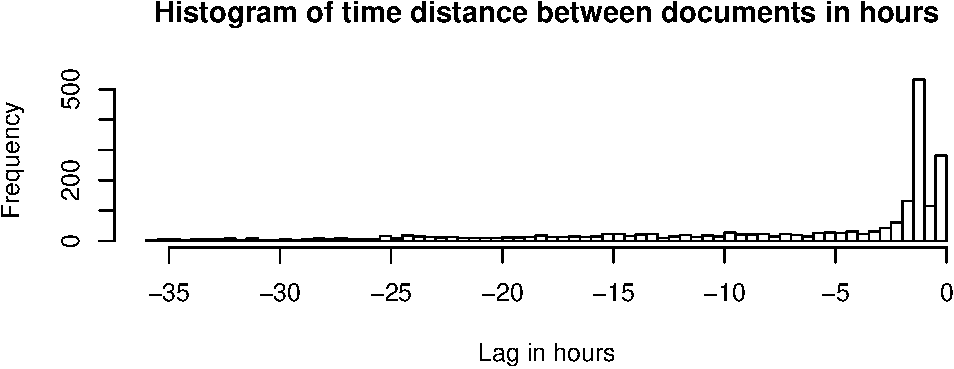
\includegraphics{newsflow_files/figure-latex/unnamed-chunk-11-1} \end{Schunk}

In the histogram we see that most document pairs with a similarity score
above the threshold are about an hour apart (-1 on the x-axis). This is
mainly because the online newspapers often follow the news agency within
a very short amount of time\footnote{Actually, many of the newspapers
  publish nearly simultaneous with the news agency. Since we had reason
  to believe that the time stamps of our news agency data were
  occasionally later than the actual publication time, we subtracted one
  hour from its publication time in general.}. As time distance
increases, the number of document pairs decreases, which makes sense
because news gets old fast, so news diffusion should occur within a
limited time after publication.

\subsection{Tailoring the document comparison window}

If news diffuses from one source to another, then the time difference
cannot be zero, since the source that follows needs time to edit and
publish the news. This delay period can also differ between sources.
Websites can adopt news within minutes, but newspapers have a long time
between pressing and publishing the newspaper, meaning that there is a
period of several hours before publication during which influence is not
possible. Thus, we have to adjust the window for document pairs. To make
it more convenient to adjust and inspect the window settings for
different sources, we offer the \texttt{filter.window} and
\texttt{show.window} functions.

The \texttt{filter.window} function can be used to filter the document
pairs (i.e.~edges) using the \texttt{hour.window} parameter, which works
identical to the \texttt{hour.window} parameter in the
\texttt{documents.window.compare} function. In addition, the
\texttt{select.vertices} parameter can be used to select the vertices
(i.e.~documents) for which this filter is applied. This makes it easy to
tailor the window for different sources, especially if the sourcetype is
included in the vertex information.

\begin{Schunk}
\begin{Sinput}
# set window for all vertices
g = filter.window(g, hour.window = c(-36, -0.1))

# set window for print newspapers
is.print = V(g)$sourcetype == 'Print NP'
g = filter.window(g, hour.window = c(-36, -6), select.vertices=is.print)
\end{Sinput}
\end{Schunk}

For all sources the window has now been adjusted so that a document can only match a document that occured at least 0.1 hours earlier.
But for print newspapers, this is more specifically set to 6 hours.
With the `show.window` function we can view the actual window in the data. 
A vertex.attribute can also be given to view the window separately for the unique values of this attribute.

\begin{Schunk}
\begin{Sinput}
show.window(g, vertex.attribute = 'source')
\end{Sinput}
\begin{Soutput}
#>   vertex.attribute window.left window.right
#> 1       Newsagency         -35        -0.15
#> 2      Online NP 1         -36        -0.10
#> 3      Online NP 2         -36        -0.12
#> 4       Print NP 1         -36        -7.02
#> 5       Print NP 2         -35        -7.35
\end{Soutput}
\end{Schunk}

\section{Analyzing the document similarity network}

Before we aggregate the network, it can be informative to look at the individual sub-components.
If a threshold for document similarity is used, then there should be multiple disconnected components of documents that are only similar to each other.
With the current data, these components tend to reflect documents that address the same or related events. 
Decomposing the network can be done with the `decompose.graph()` function from the `igraph` package.

\begin{Schunk}
\begin{Sinput}
g_subcomps = decompose.graph(g)
length(g_subcomps)
\end{Sinput}
\begin{Soutput}
#> [1] 658
\end{Soutput}
\end{Schunk}

The current data has 658 sub-components. 
To visualize these components, we offer the `plot.document.network` function.
This function draws a network where nodes (i.e. documents) are positioned based on their date (x-axis) and source (y-axis).

\begin{Schunk}
\begin{Sinput}
gs = g_subcomps[[2]] # select the second sub-component
plot.document.network(gs)
\end{Sinput}

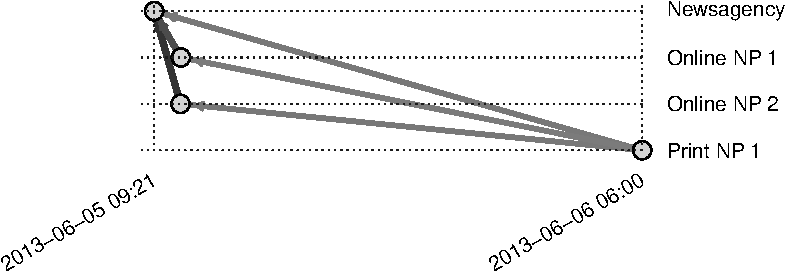
\includegraphics{newsflow_files/figure-latex/unnamed-chunk-15-1} \end{Schunk}

The visualization shows that a news message was first published by the news agency on June 5th around 9 AM. 
Soon after this messages was adopted by two online newspapers, and later on also by a print newspaper.
The grayscale and width of the edges also show that the online newspaper messages were very similar (i.e. thick and black) to the news agency message.

By default, the "source" attribute is used for the y-axis, but this can be changed to other document attributes using the `source.attribute` parameters.
If a DTM is also provided, the visualization will also include a word cloud with the most frequent words of these documents.

\begin{Schunk}
\begin{Sinput}
plot.document.network(gs, source.attribute = 'sourcetype', dtm=dtm)
\end{Sinput}

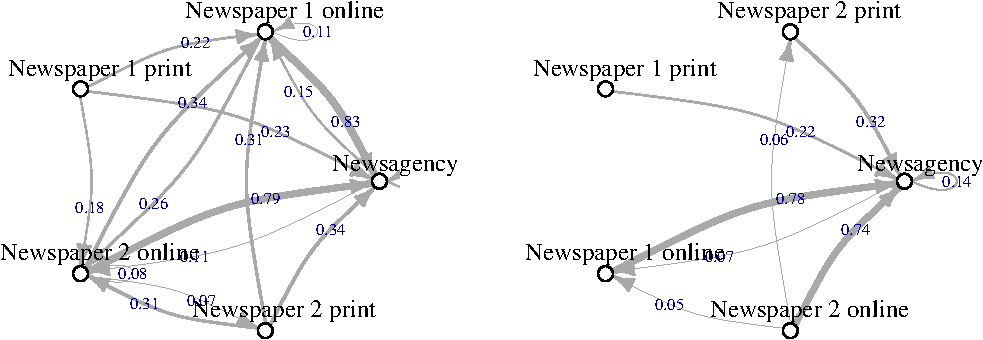
\includegraphics{newsflow_files/figure-latex/unnamed-chunk-16-1} \end{Schunk}

These visualizations and the corresponding subcomponents help us to qualitatively investigate specific cases. 
This also helps to evaluate how well the document similarity measures are valid given the goal of the analysis.
Furthermore, they illustrate how we can analyze homogeneity and news diffusion patterns.
For each source we can count what proportion of its publications is similar to earlier publications by specific other sources.
We can also analyze the average time between publications.

Another usefull application is that we can use them to see whether certain transformation of the network might be required.
Depending on the purpose of the analysis it can be relevant to add or delete certain edges.
For instance, in the previous visualizations we see that a print newspaper message matched both a recent newsagency message and two online newspaper messages.
If we are specifically interested in who the original source of the message is, then it makes sense to only count the edge to the newsagency.
Thus, we can develop functions to transform the network to enable such alternative types of analysis.
Here we demonstrate the `only.first.match` function, which transforms the network so that a document only has an edge to the earliest dated document it matches within the specified time window.

\begin{Schunk}
\begin{Sinput}
gs_onlyfirst = only.first.match(gs)
plot.document.network(gs_onlyfirst)
\end{Sinput}

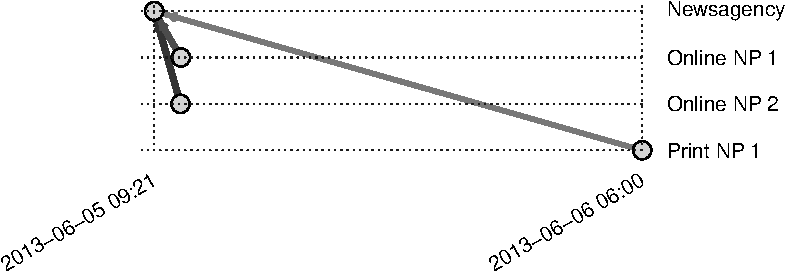
\includegraphics{newsflow_files/figure-latex/unnamed-chunk-17-1} \end{Schunk}

\subsection{Aggregating the document similarity network}

This package offers the  `aggregate.network` function as a versatile way to aggregate the edges of the document similarity network based on the vertex attributes (i.e. the document meta information).
The first argument is the network (in the `igraph` class). 
The second argument, for the `by` parameter, is a character vector to indicate one or more vertex attributes based on which the edges are aggregated.
Optionally, the `by` characteristics can also be specified separately for `by.from` and `by.to`. 
This gives flexible control over the data, for instance to look at source and sourcetypes, or to aggregate scores per month.

By default, the function returns the number of edges, as well as the number of nodes that is connected for both the `from` and `to` group. 
These values are relevant if a threshold for similarity (edge weight) is used, so that whether or not an edge exists indicates whether or not two documents are similar.
In addition, if an `edge.attribute` is given, this attribute will be aggregated using the function specified in `agg.FUN`.
For the following example we include this to analyze the median of the `hourdiff` attribute.

\begin{Schunk}
\begin{Sinput}
g.agg = aggregate.network(g, by='source', edge.attribute='hourdiff', agg.FUN=median)

e = get.data.frame(g.agg, 'edges')
head(e)
\end{Sinput}
\begin{Soutput}
#>          from          to edges agg.hourdiff from.V from.Vprop to.V
#> 1  Newsagency  Newsagency   124         -8.1     95       0.16  112
#> 2 Online NP 1  Newsagency   451         -1.3    384       0.83  425
#> 3 Online NP 2  Newsagency   379         -1.3    330       0.79  374
#> 4  Print NP 2  Newsagency    60        -15.9     45       0.34   60
#> 5  Print NP 1  Newsagency    38        -16.6     34       0.23   38
#> 6  Newsagency Online NP 1   107         -4.8     91       0.15   90
#>   to.Vprop
#> 1    0.188
#> 2    0.712
#> 3    0.626
#> 4    0.101
#> 5    0.064
#> 6    0.195
\end{Soutput}
\end{Schunk}

In the edges of the aggregated network there are six scores for each edge. 
The `edges` attribute counts the number of edges from the `from` group to the `to` group. 
For example, we see that \emph{online NP 1} documents have 451 edges to \emph{newsagency} documents.
The `agg.hourdiff` attribute shows that the median of the hourdiff attribute of these 451 edges is -1.27 (1 hour and 16 minutes).
In addition to the edges, we can look at the number of vertices (i.e. documents) in the `from` group that matched with at least one vertex in the `to` group. 
This is given by the `from.V` attribute, which shows here that 384 \emph{online NP 1} documents matched with a \emph{newsagency} document$[^lowerthanedges]$.
This is also given as the proportion of all vertices/documents in the `from` group, as the `from.Vprop` attribute.
Substantially, the `from.Vprop` score thus indicates that 83.12% of political news messages in \emph{online NP 1} is similar or identical to recent \emph{newsagency} messages.
For the analysis of content homogeneity and news diffusion, the `from.Vprop` attribute is often most relevant.

The `V' and 'Vprop` scores are also reported for the `to` group. 
This gives an inversed perspective on the relation between the `from` and `to` groups.
Based on the `to.V` score, we see that 71.12% of documents published by the \emph{newsagency} is similar or identical to future documents in \emph{online NP 1}.
In other words, of all the political news messages published by the \emph{newsagency}, 71.12% was afterwards also published by \emph{online NP 1}.
Thus, `from.Vprop` and `to.Vprop` are related but different scores, and can be used to answer different research questions.

$[^lowerthanedges]:$ Note that the `edges` score is always equal to or higher than the `from.matched` score, since one document can match with multiple other documents. 

\subsection{Inspecting and visualizing results}

We already saw that the network data can be transformed to a common data.frame with the `get.data.frame` function.
Alternatively, `igraph` has the `get.adjacency` function to return the values for one edge attribute as a matrix with the vertices in the rows and columns.

\begin{Schunk}
\begin{Sinput}
get.adjacency(g.agg, attr= 'from.Vprop', sparse = F)
\end{Sinput}
\begin{Soutput}
#>             Newsagency Online NP 1 Online NP 2 Print NP 2 Print NP 1
#> Newsagency        0.16        0.15       0.109     0.0168      0.030
#> Online NP 1       0.83        0.11       0.264     0.0260      0.045
#> Online NP 2       0.79        0.34       0.077     0.0743      0.041
#> Print NP 2        0.34        0.31       0.305     0.0076      0.015
#> Print NP 1        0.23        0.22       0.184     0.0068      0.027
\end{Soutput}
\end{Schunk}

Furthermore, we can use the network visualization features of the `igraph` package. 
This can help present the document similarity data in an easily interpretable way.
For this example we use a threshold of 0.2 for `from.Vprop`.

\begin{Schunk}
\begin{Sinput}
g.agg.thres = delete.edges(g.agg, which(E(g.agg)$from.Vprop < 0.2))
plot(g.agg.thres, layout=layout.circle, 
     edge.width = E(g.agg.thres)$from.Vprop*5, 
     edge.label = round(E(g.agg.thres)$from.Vprop,2), 
     edge.curved=0.3, edge.label.cex=0.8, vertex.label.dist=0.8)
\end{Sinput}


\begin{center}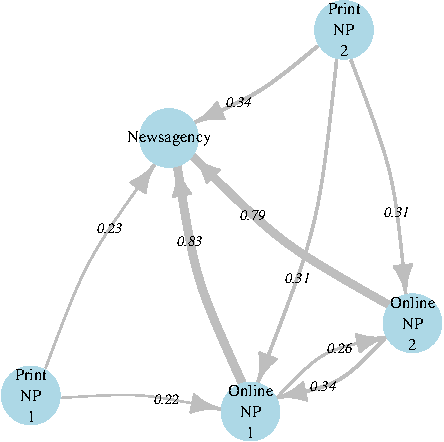
\includegraphics{newsflow_files/figure-latex/unnamed-chunk-20-1} \end{center}

\end{Schunk}

For illustration, we can now see how the results change if we transform
the network with the \texttt{only.first.match} function, which only
counts edges to the first source that published a document.

\begin{Schunk}
\begin{Sinput}
g2 = only.first.match(g)
g2.agg = aggregate.network(g2, by='source', edge.attribute='hourdiff', agg.FUN=median)

g2.agg.thres = delete.edges(g2.agg, which(E(g2.agg)$from.Vprop < 0.2))
plot(g2.agg.thres, layout=layout.circle, 
     edge.width = E(g2.agg.thres)$from.Vprop*5, 
     edge.label = round(E(g2.agg.thres)$from.Vprop,2), 
     edge.curved=0.3, edge.label.cex=0.8, vertex.label.dist=0.8)
\end{Sinput}


\begin{center}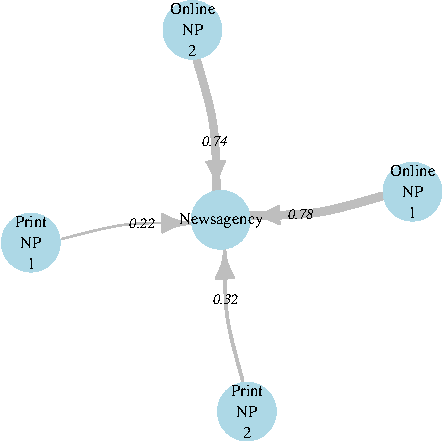
\includegraphics{newsflow_files/figure-latex/unnamed-chunk-21-1} \end{center}

\end{Schunk}

The first network is much more dense compared to the second.
In particular, we see stronger edges between the print and online editions of the newspapers.
In the second network almost only the ties to the news agency remain.
This implies that many of the edges between newspapers in the first network resulted from cases where both newspapers adopt the same news agency articles.

Note, however, that the second network is not better per se.
It is possible that the initial source of a message is not the direct source.
For example, a blog might not have acces to the news agency feed, and therefore only receive news agency messages if they are published by another source.
Thus, the most suitable approach depends on the purpose of the analysis.
One of the goals of this package is to develop best practises for different occasions.

\subsection{Alternative applications of this package}

There are several alternative applications of the functions offered in this package that are not covered in this vignette. 
Here we briefly point out some of the more usefull alternatives.

In the aggregate.network function it is possible to use different vertex attributes to aggregate the edges for `from` and `to` nodes.
A particularlly interesting application of this feature is to use the publication date in the aggregation.
For instance, with the following settings, we can get the proportion of matched documents per day.
Here we also use the `return.df` parameter in the `aggregate.network` function, to directly return the results as a data.frame. 

\begin{Schunk}
\begin{Sinput}
V(g)$day = format(as.Date(V(g)$date), '%Y-%m-%d')
agg.perday = aggregate.network(g, by.from=c('source', 'day'), by.to='source', 
                                  edge.attribute='hourdiff', agg.FUN=median, 
                                  return.df=T)

head(agg.perday)
\end{Sinput}
\begin{Soutput}
#>    to.source from.source   from.day edges agg.hourdiff from.V to.V
#> 1 Newsagency  Newsagency 2013-06-01     1         -9.7      1    1
#> 2 Newsagency  Print NP 2 2013-06-06     2        -26.1      1    2
#> 3 Newsagency Online NP 1 2013-06-09     9         -1.2      7    9
#> 4 Newsagency  Print NP 2 2013-06-22     2        -20.3      2    2
#> 5 Newsagency  Newsagency 2013-06-02     1        -28.7      1    1
#> 6 Newsagency  Newsagency 2013-06-03     2         -3.5      2    1
#>   from.Vprop to.Vprop
#> 1      0.100   0.0017
#> 2      0.333   0.0034
#> 3      0.875   0.0151
#> 4      0.333   0.0034
#> 5      0.200   0.0017
#> 6      0.091   0.0017
\end{Soutput}
\end{Schunk}

This way the aggregated document similarity data can be analyzed as a time-series. 
For instance, to analyze whether certain developments affect content homogeneity or intermedia dynamics. 
Also, it enables us to analyze the mean of the aggregated results over time. 
The `return.df` feature is convenient for this purpose, because it directly matches all the vertex and edge attributes (as opposed to the `get.data.frame` function).

Another usefull application of this feature is to only aggregate the `by.to` nodes, by using the vertex name in the `by.from` argument. 
This way, the data can easily be matched to data on content characteristics of individual documents.
For instance, to analyze whether certain elements of documents predict whether or not the message is also covered by other sources.
In addition, we set the `edge.attribute` to "weight" and `agg.FUN` to max, so that for each document we can see how strong the strongest match with each source was. 

\begin{Schunk}
\begin{Sinput}
agg.perdoc = aggregate.network(g, by.from='name', by.to='sourcetype', 
                                  edge.attribute='weight', agg.FUN=max, 
                                  return.df=T)

docXsource = xtabs(agg.weight ~ from.name + to.sourcetype, agg.perdoc, sparse = F)
head(docXsource)
\end{Sinput}
\begin{Soutput}
#>            to.sourcetype
#> from.name   Newsagency Online NP Print NP
#>   147908495       0.00      0.00     0.52
#>   150454037       0.00      0.00     0.43
#>   150454094       0.00      0.42     0.00
#>   150454110       0.40      0.00     0.00
#>   150454132       0.54      0.54     0.00
#>   150454155       0.00      0.00     0.42
\end{Soutput}
\end{Schunk}

Finally, note that we have now only compared documents to prior documents. 
We thereby focus the analysis on whether each document is potentially influenced by certain other documents.
By changing the window setting, it is also possible to compare each document to both prior and future documents, to focus on content homogeneity.
Or to compare only to future documents, to shift the focus to influence (what messages become adopted) instead of dependence (what messages were adopted from others).

\section{Conclusion and future improvements}

We have demonstrated how the \emph{newsflow} package can be used to perform a many-to-many comparison of documents.
The primary focus and most important feature of this package is the `documents.window.compare` function.
This function compares all documents that occur within a given time distance, which makes it computationally feasible for longitudinal data.
Using this data, we can analyze to what extent different sources publish the same content and whether there are consistent patterns in who follows whom.
The secondary focus of this package is to provide functions to conduct this analysis, and to provide a platform for scholars to share additional or alternative approaches.

The data input required for this analysis consists solely of textual documents and their corresponding publication date and source.
Since no human coding is required, the package enables large scale comparative and longitudinal studies.
Although the demonstration in this vignette used a moderate sized dataset, the `document.window.compare` can handle much larger data and is fast, thanks to the excellent sparse matrix multiplication alghoritm of the `Matrix` package.

The goal is to continue developing this package as a specialized toolkit for analyzing the homogeneity and diffusion of news content.
First of all, additional approaches for measuring whether documents are related will be added.
Currently only a vector space model approach for calculating document similarity is implemented.
For future versions alternative approaches such as language modeling will also be explored.
In particular, we want to add alternative measures to express the relation of documents over time in terms of probability and information gain.
This would also allow us to define a more formal way to determine whether or not a relation exists, other than using a constant threshold.
Secondly, new methods for analyzing and visualizing the network data will be explored. 
In particular, methods will be implemented for analyzing patterns beyond dyadic ties between news outlets, building on techniques from the field of network analysis.
To promote the involvement of other scholars and professionals in this development, the package is published entirely open-source. 
The source code is hosted on GitHub--\emph{https://github.com/kasperwelbers/newsflow}.

\section{Practical code example}

\begin{Schunk}
\begin{Sinput}
# Prepare DTM and meta data
data(dtm)
data(meta)

tdd = term.day.dist(dtm, meta)
dtm = dtm[,tdd$term[tdd$days.entropy.norm <= 0.3]]

dtm = weightTfIdf(dtm)

# Prepare document similarity network
g = documents.window.compare(dtm, meta, hour.window = c(-36,-0.1), min.similarity = 0.4)
g = filter.window(g, hour.window = c(-36, -6), V(g)$sourcetype == 'Print NP')

# Aggregate network 
g.agg = aggregate.network(g, by='source', edge.attribute='hourdiff', agg.FUN=median)

get.adjacency(g.agg, attr='from.Vprop')
get.data.frame(g.agg, 'edges')
\end{Sinput}
\end{Schunk}

\section{References}

\address{
Kasper Welbers\\
VU University Amsterdam\\
De Boelelaan 1081,\\ 1081 HV Amsterdam, The Netherlands\\
}
\href{mailto:k.welbers@vu.nl}{\nolinkurl{k.welbers@vu.nl}}

\address{
Wouter van Atteveldt\\
VU University Amsterdam\\
De Boelelaan 1081,\\ 1081 HV Amsterdam, The Netherlands\\
}
\href{mailto:wouter@vanatteveldt.com}{\nolinkurl{wouter@vanatteveldt.com}}

